% ========================================
%	Header einbinden
% ========================================

\documentclass[bibtotoc,titlepage]{scrartcl}

% Deutsche Spracheinstellungen
\usepackage[ngerman,german]{babel, varioref}
\usepackage[T1]{fontenc}
\usepackage[utf8]{inputenc}

%\usepackage{marvosym}

\usepackage{amsfonts}
\usepackage{amssymb}
\usepackage{amsmath}
\usepackage{amscd}
\usepackage{amstext}
\usepackage{float}
\usepackage{caption}
\usepackage{wrapfig}
\usepackage{setspace}
\usepackage{threeparttable}
\usepackage{footnote}

\usepackage{caption}
\usepackage{subcaption}

\newfloat{formel}{htbp}{for}
\floatname{formel}{Formel}


\usepackage{longtable}

%\usepackage{bibgerm}

\usepackage{footnpag}

\usepackage{ifthen}                 %%% package for conditionals in TeX
\usepackage{siunitx}
%Fr textumflossene Bilder und Tablellen
%\usepackage{floatflt} - veraltet

%Fr Testzwecke aktivieren, zeigt labels und refs im Text an.
%\usepackage{showkeys}

% Abstand zwischen zwei Abs�zen nach DIN (1,5 Zeilen)
% \setlength{\parskip}{1.5ex plus0.5ex minus0.5ex}

% Einrckung am Anfang eines neuen Absatzes nach DIN (keine)
%\setlength{\parindent}{0pt}

% R�der definieren
% \setlength{\oddsidemargin}{0.3cm}
% \setlength{\textwidth}{15.6cm}

% bessere Bildunterschriften
%\usepackage[center]{caption2}


% Probleml�ungen beim Umgang mit Gleitumgebungen
\usepackage{float}

% Nummeriert bis zur Strukturstufe 3 (also <section>, <subsection> und <subsubsection>)
%\setcounter{secnumdepth}{3}

% Fhrt das Inhaltsverzeichnis bis zur Strukturstufe 3
%\setcounter{tocdepth}{3}

\usepackage{exscale}

\newenvironment{dsm} {\begin{displaymath}} {\end{displaymath}}
\newenvironment{vars} {\begin{center}\scriptsize} {\normalsize \end{center}}


\newcommand {\en} {\varepsilon_0}               % Epsilon-Null aus der Elektrodynamik
\newcommand {\lap} {\; \mathbf{\Delta}}         % Laplace-Operator
\newcommand {\R} { \mathbb{R} }                 % Menge der reellen Zahlen
\newcommand {\e} { \ \mathbf{e} }               % Eulersche Zahl
\renewcommand {\i} { \mathbf{i} }               % komplexe Zahl i
\newcommand {\N} { \mathbb{N} }                 % Menge der nat. Zahlen
\newcommand {\C} { \mathbb{C} }                 % Menge der kompl. Zahlen
\newcommand {\Z} { \mathbb{Z} }                 % Menge der kompl. Zahlen
\newcommand {\limi}[1]{\lim_{#1 \rightarrow \infty}} % Limes unendlich
\newcommand {\sumi}[1]{\sum_{#1=0}^\infty}
\newcommand {\rot} {\; \mathrm{rot} \,}         % Rotation
\newcommand {\grad} {\; \mathrm{grad} \,}       % Gradient
\newcommand {\dive} {\; \mathrm{div} \,}        % Divergenz
\newcommand {\dx} {\; \mathrm{d} }              % Differential d
\newcommand {\cotanh} {\; \mathrm{cotanh} \,}   %Cotangenshyperbolicus
\newcommand {\asinh} {\; \mathrm{areasinh} \,}  %Area-Sinus-Hyp.
\newcommand {\acosh} {\; \mathrm{areacosh} \,}  %Area-Cosinus-H.
\newcommand {\atanh} {\; \mathrm{areatanh} \,}  %Area Tangens-H.
\newcommand {\acoth} {\; \mathrm{areacoth} \,}  % Area-cotangens
\newcommand {\Sp} {\; \mathrm{Sp} \,}
\newcommand {\mbe} {\stackrel{\text{!}}{=}}     %Must Be Equal
\newcommand{\qed} { \hfill $\square$\\}
\renewcommand{\i} {\imath}
\def\captionsngerman{\def\figurename{\textbf{Abb.}}}

%%%%%%%%%%%%%%%%%%%%%%%%%%%%%%%%%%%%%%%%%%%%%%%%%%%%%%%%%%%%%%%%%%%%%%%%%%%%
% SWITCH FOR PDFLATEX or LATEX
%%%%%%%%%%%%%%%%%%%%%%%%%%%%%%%%%%%%%%%%%%%%%%%%%%%%%%%%%%%%%%%%%%%%%%%%%%%%
%%%
\ifx\pdfoutput\undefined %%%%%%%%%%%%%%%%%%%%%%%%%%%%%%%%%%%%%%%%% LATEX %%%
%%%
\usepackage[dvips]{graphicx}       %%% graphics for dvips
\DeclareGraphicsExtensions{.eps,.ps}   %%% standard extension for included graphics
\usepackage[ps2pdf]{thumbpdf}      %%% thumbnails for ps2pdf
\usepackage[ps2pdf,                %%% hyper-references for ps2pdf
bookmarks=true,%                   %%% generate bookmarks ...
bookmarksnumbered=true,%           %%% ... with numbers
hypertexnames=false,%              %%% needed for correct links to figures !!!
breaklinks=true,%                  %%% breaks lines, but links are very small
linkbordercolor={0 0 1},%          %%% blue frames around links
pdfborder={0 0 112.0}]{hyperref}%  %%% border-width of frames
%                                      will be multiplied with 0.009 by ps2pdf
%
%\hypersetup{ pdfauthor   = {Hannes Franke; Julius Tilly},
%pdftitle    = {x}, pdfsubject  = {Protokoll FP}, pdfkeywords = {V301, Innenwiderstand, Leistungsanpassung},
%pdfcreator  = {LaTeX with hyperref package}, pdfproducer = {dvips
%+ ps2pdf} }
%%%
\else %%%%%%%%%%%%%%%%%%%%%%%%%%%%%%%%%%%%%%%%%%%%%%%%%%%%%%%%%% PDFLATEX %%%
%%%
\usepackage[pdftex]{graphicx}      %%% graphics for pdfLaTeX
\DeclareGraphicsExtensions{.pdf}   %%% standard extension for included graphics
\usepackage[pdftex]{thumbpdf}      %%% thumbnails for pdflatex
\usepackage[pdftex,                %%% hyper-references for pdflatex
bookmarks=true,%                   %%% generate bookmarks ...
bookmarksnumbered=true,%           %%% ... with numbers
hypertexnames=false,%              %%% needed for correct links to figures !!!
breaklinks=true,%                  %%% break links if exceeding a single line
linkbordercolor={0 0 1},
linktocpage]{hyperref} %%% blue frames around links
%                                  %%% pdfborder={0 0 1} is the default
% \hypersetup{
% pdftitle    = {V301 Innenwiderstand und Leistungsanpassung}, 
% pdfsubject  = {Protokoll AP}, 
% pdfkeywords = {V301, Innenwiderstand, Leistungsanpassung},
% pdfsubject  = {Protokoll AP},
% pdfkeywords = {V301, Innenwiderstand, Leistungsanpassung}}
%                                  %%% pdfcreator, pdfproducer,
%                                      and CreationDate are automatically set
%                                      by pdflatex !!!
\pdfadjustspacing=1                %%% force LaTeX-like character spacing
\usepackage{epstopdf}
%
\fi %%%%%%%%%%%%%%%%%%%%%%%%%%%%%%%%%%%%%%%%%%%%%%%%%%% END OF CONDITION %%%
%%%%%%%%%%%%%%%%%%%%%%%%%%%%%%%%%%%%%%%%%%%%%%%%%%%%%%%%%%%%%%%%%%%%%%%%%%%%
% seitliche Tabellen und Abbildungen
%\usepackage{rotating}
\usepackage{ae}
\usepackage{
  array,
  booktabs,
  dcolumn
}
\makeatletter 
  \renewenvironment{figure}[1][] {% 
    \ifthenelse{\equal{#1}{}}{% 
      \@float{figure} 
    }{% 
      \@float{figure}[#1]% 
    }% 
    \centering 
  }{% 
    \end@float 
  } 
  \makeatother 


  \makeatletter 
  \renewenvironment{table}[1][] {% 
    \ifthenelse{\equal{#1}{}}{% 
      \@float{table} 
    }{% 
      \@float{table}[#1]% 
    }% 
    \centering 
  }{% 
    \end@float 
  } 
  \makeatother 
%\usepackage{listings}
%\lstloadlanguages{[Visual]Basic}
%\allowdisplaybreaks[1]
%\usepackage{hycap}
%\usepackage{fancyunits}

% ========================================
%	Angaben für das Titelblatt
% ========================================

\title{Debye-Scherrer Aufnahmen\\				% Titel des Versuchs 
\large TU Dortmund, Fakultät Physik\\ 
\normalsize Fortgeschrittenen-Praktikum}

\author{Jan Adam\\			% Name Praktikumspartner A
{\small \href{jan.adam@tu-dortmund.de}{jan.adam@tu-dortmund.de}}	% Erzeugt interaktiven einen Link
\and						% um einen weiteren Author hinzuzfügen
Dimitrios Skodras\\					% Name Praktikumspartner B
{\small \href{dimitrios.skodras@tu-dortmund.de}{dimitrios.skodras@tu-dortmund.de}}		% Erzeugt interaktiven einen Link
}
\date{31. Oktober 2016}				% Das Datum der Versuchsdurchführung

% ========================================
%	Das Dokument beginnt
% ========================================

\begin{document}

% ========================================
%	Titelblatt erzeugen
% ========================================

\maketitle					% Jetzt wird die Titelseite erzeugt
\thispagestyle{empty} 				% Weder Kopfzeile noch Fußzeile

% ========================================
%	Der Vorspann
% ========================================

%\newpage					% Wenn Verzeichnisse auf einer neuen Seite beginnen sollen
%\pagestyle{empty}				% Weder Kopf- noch Fußzeile für Verzeichnisse

\tableofcontents

%\newpage					% eine neue Seite
%\thispagestyle{empty}				% Weder Kopf- noch Fußzeile für Verzeichnisse
%\listoffigures					% Abbildungsverzeichnis

%\newpage					% eine neue Seite
%\thispagestyle{empty}				% Weder Kopf- noch Fußzeile für Verzeichnisse
%\listoftables					% Tabellenverzeichnis
\newpage					% eine neue Seite


% ========================================
%	Kapitel
% ========================================

%\section{Einleitung}				% Bei Bedarf

\section{Theorie}\label{sec:theorie}
Viele makroskopische Eigenschaften von Materie können auf den Aufbau ihrer Grundbausteine, dh. Atome und Moleküle zurückgeführt werden. Bei den für diesen Versuch vorliegenden Proben liegen diese in kristalliner Form vor und bilden regelmäßig auftretende Strukturen, sog. Gitter aus. Durch die Untersuchung dieser Gitter können wichtige tensorielle und vektorielle makroskopische Eigenschaften, wie zum Beispiel Elastizität und Permeabilität bestimmt werden. Um die Gitterabstände auflösen zu können, die im $\mathring{A}$ngströmbereich liegen, ist die Wellenlänge des sichtbaren Lichtes zu groß. Röntgenstrahlen haben jedoch das benötigte Auflösungsvermögen und ermöglichen eine Untersuchung der Strukturen.

\subsection{Über die Struktur der Materie}
Wie in Kapitel \ref{sec:theorie} erwähnt, liegen die Atome von Festkörpern in Gitterstruktur vor. Diese können durch einen Translationsvektor
\begin{align}
	\vec{t} = n_1\vec{a} +n_2\vec{b} + n_3\vec{c}
\end{align}
beschrieben werden, der ausgehend von einem Startpunkt auf alle anderen Gitterpunkte zeigt, wenn man für die $n_i$ ganze Zahlen einsetzt. An den Gitterpunkten können entweder einzelne oder mehrere Atome sitzen. Diese Ansammlungen nennt man Basis. 

Hinsichtlich ihrer Symmetrieeigenschaften werden die dreidimensionalen Gitter in 14 Gitterstrukturen zusammengefasst, den sog. Bravais-Gittern. Diese sind in 7 Gittersysteme unterteilt: triklin, monoklin, (ortho-)rhombisch, tetragonal, rhomboedrisch, hexagonal und kubisch. Alle Systeme und ihre Eigenschaften sind in Abbildung \ref{pic:bravais} aufgelistet.
\begin{figure}[htbp]
	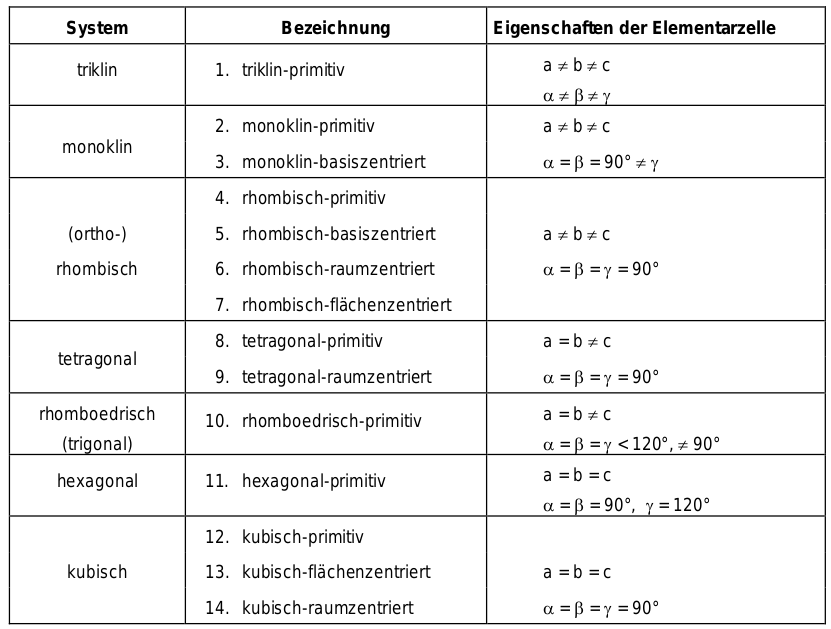
\includegraphics[width=0.9\textwidth]{../pics/bravais.png}
	\caption{Auflistung der 14 Bravaisgitter im dreidimensionalen Raum \cite{Anleitung}.}
	\label{pic:bravais}
\end{figure}

Besonderes Interesse  kommt dabei der sog. Elementarzelle zu. Dies ist die kleinste Einheit, die eine Kristallstruktur vollkommen festlegt. Beispielsweise kann man dazu das von den Vektoren $\vec{a}$, $\vec{b}$ und $\vec{c}$ aufgespannte Parallelepiped benutzen. Liegen nur auf den Eckpunkten Atome, enthält die Zelle also im Ganzen nur ein einzelnes Atom, so nennt man sie primitive Elementarzelle. 
Nicht jede Kristallstruktur lässt sich jedoch durch Vervielfachung einer primitiven Elementarzelle aufbauen. Die in diesem Versuch untersuchten Stoffe haben eine kubische Grundstruktur, daher wird nur dieses System im Folgenden detaillierter beschrieben. Neben dem kubisch-primitiven Gitter, welches nur in den 8 Eckpunkten des Parallelepipeds Atome sitzen hat, gibt es noch das kubisch-raumzentrierte und das kubisch-flächenzentrierte Gitter. Diese werden in Abbildung \ref{pic:gitterTyp1} dargestellt.

\begin{figure}[htbp]
	\centering
	\begin{subfigure}[b]{0.3\textwidth}
		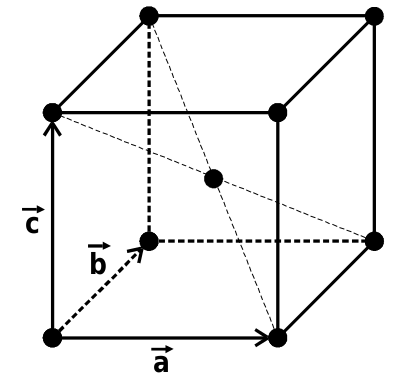
\includegraphics[width=\textwidth]{../pics/bcc.png}
		\caption{bcc-Gitter}
		\label{pic:bcc}
	\end{subfigure}
	~ %add desired spacing between images, e. g. ~, \quad, \qquad, \hfill etc.
	%(or a blank line to force the subfigure onto a new line)
	\begin{subfigure}[b]{0.3\textwidth}
		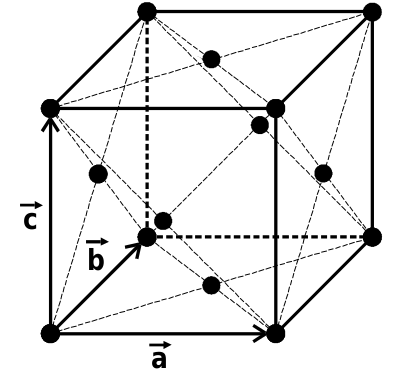
\includegraphics[width=\textwidth]{../pics/fcc.png}
		\caption{fcc-Gitter}
		\label{pic:fcc}
	\end{subfigure}
	\caption{Darstellung des kubisch-raumzentrierten und kubisch-flächenzentrierten Gitters. Es befindet sich ein weiteres Atom im inneren der Elementarzelle bzw. je eines in den Mitten der Würfelflächen \cite{Anleitung}.}
	\label{pic:gitterTyp1}
\end{figure}
Das kubisch-raumzentrierte Gitter (Abb. \ref{pic:bcc}) enthält zusätzlich zu den Atomen an den Eckpunkten noch ein weiteres im Zentrum. Damit ist es keine primitive Einheitszelle mehr, da die Zelle insgesamt 2 Atome enthält. Bei der kubisch-flächenzentrierten Zelle (Abb. \ref{pic:fcc}) sitzt dagegen auf jeder Flächenmitte ein weiteres Atom, wodurch die Einheitszelle sogar 4 Atome enthält.

Beschrieben werden diese verschiedenen Zelltypen durch die Position der Atome in der Basiszelle. Im Falle der primitiven Einheitszellen wäre dies lediglich ein Atom: $(0,0,0)$, im \textbf{bcc Gitter} zwei Atome: $(0,0,0)$ und $(\nicefrac{1}{2},\nicefrac{1}{2},\nicefrac{1}{2})$ und im \textbf{fcc Gitter} vier Atome: $(0,0,0)$, $(0,\nicefrac{1}{2},\nicefrac{1}{2})$, $(\nicefrac{1}{2},0,\nicefrac{1}{2})$ und $(\nicefrac{1}{2},\nicefrac{1}{2},0)$.\\

\begin{figure}[htbp]
	\centering
	\begin{subfigure}[b]{0.3\textwidth}
		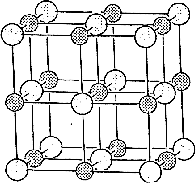
\includegraphics[width=\textwidth]{../pics/steinsalz.png}
		\caption{Steinsalzstruktur}
		\label{pic:steinsalz}
	\end{subfigure}
	~ %add desired spacing between images, e. g. ~, \quad, \qquad, \hfill etc.
	%(or a blank line to force the subfigure onto a new line)
	\begin{subfigure}[b]{0.3\textwidth}
		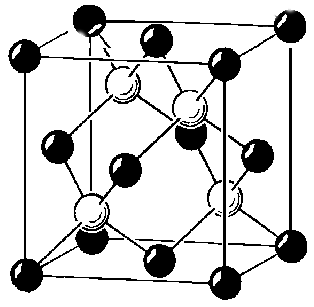
\includegraphics[width=\textwidth]{../pics/zinkblende.png}
		\caption{Zinkblendenstruktur}
		\label{pic:zinkblende}
	\end{subfigure}
	\caption{Darstellung der Steinsalz- und Zinkblendenstruktur. Das Steinsalzgitter besteht aus zwei um eine halbe Raumdiagonale zu einander verschobenen fcc-Gittern, mit verschiedenen Atomsorten; beispielsweise Na und Cl in Natriumchlorid.\\
	Die Zinkblendenstruktur besteht ebenfalls aus zwei fcc Gittern, die jedoch um eine viertel Raumdiagonale zueinander verschoben sind. Ein Beispiel ist Zinksulfid \cite{Anleitung}.}
	\label{pic:gitterTyp2}
\end{figure}
Für die durchgeführte Messung ebenfalls von Bedeutung sind:

Die \textbf{Steinsalzstruktur}, über die beispielsweise NaCl verfügt. Sie besteht aus zwei fcc Gittern, die mit unterschiedlichen Atomsorten bestückt sind und deren Ursprünge um $(\nicefrac{1}{2},\nicefrac{1}{2},\nicefrac{1}{2})$ gegeneinander verschoben sind.

Die \textbf{Diamantstruktur}, die aus zwei um ein viertel einer Raumdiagonalen zueinander verschobenen fcc-Gittern besteht. Die Atome liegen also an den Orten  $(0,0,0)$, $(\nicefrac{1}{2},\nicefrac{1}{2},0)$, $(\nicefrac{1}{2},0,\nicefrac{1}{2})$, $(0,\nicefrac{1}{2},\nicefrac{1}{2})$, 
$(\nicefrac{1}{4},\nicefrac{1}{4},\nicefrac{1}{4})$, $(\nicefrac{3}{4},\nicefrac{3}{4},\nicefrac{1}{4})$, $(\nicefrac{3}{4},\nicefrac{1}{4},\nicefrac{3}{4})$ und $(\nicefrac{1}{4},\nicefrac{3}{4},\nicefrac{3}{4})$.

Die \textbf{Zinkblendenstruktur}. Diese ist in Abbildung \ref{pic:zinkblende} dargestellt und entspricht einer Diamantstruktur, bei der jedoch die beiden fcc-Gitter mit verschiedenen Atomsorten besetzt sind.

Die \textbf{Cäsiumchloridstruktur}, welche aus zwei kubisch-primitiven Gittern besteht, die jeweils mit einem anderen Element, $A$ bzw. $B$, besetzt sind.
Die Gitter sind zueinander um eine halbe Raumdiagonale verschoben, sodass die Koordinaten der Atome in der Elementarzelle $A:(0,0,0)$ und $B:(\nicefrac12,\nicefrac12,\nicefrac12)$
lauten.

Die letzte hier betrachtete ist die \textbf{Fluoritstruktur}. Verbindungen mit dieser Struktur sind vom Typ $AB_2$. Alle drei Gitter sind 
kubisch-flächenzentriert und um $\nicefrac14$ bzw. $\nicefrac34$ entlang der Würfeldiagonalen zueinander verschoben. Die zwölf Atome der Elementarzelle
besetzen folgende Gitterpunkte: $A:\{(0,0,0),(\nicefrac12,\nicefrac12,0),(\nicefrac12,0,\nicefrac12),(0,\nicefrac12,\nicefrac12)\}$; 
$^1B\{(\nicefrac14,\nicefrac14,\nicefrac14),(\nicefrac34,\nicefrac34,\nicefrac14),(\nicefrac34,\nicefrac14,\nicefrac34),(\nicefrac14,\nicefrac34,\nicefrac34)\} $
und $^2B\{(\nicefrac34,\nicefrac34,\nicefrac34),(\nicefrac14,\nicefrac14,\nicefrac34),\\(\nicefrac14,\nicefrac34,\nicefrac14),(\nicefrac34,\nicefrac14,\nicefrac14) \}$.

\subsection{Netzebenen}
Eine weitere wichtige Eigenschaft von Kristallen ist die Orientierung ihrer Netzebenen und deren Abstände.
Unter einer Netzebene im Kristall versteht man eine Ebene, in der Schwerpunkte von Atomen liegen. Die Gesamtheit aller Netzebenen, die zu einer vorgegebenen parallel liegen und daher äquidistant sind, bezeichnet man als Netzebenenschar. Ihre Orientierung wird durch die sog. Millerschen Indizes beschrieben. Diese sind ein Zahlentripel (hkl) aus natürlichen Zahlen und werden wie folgt bestimmt:
\begin{figure}[htbp]
	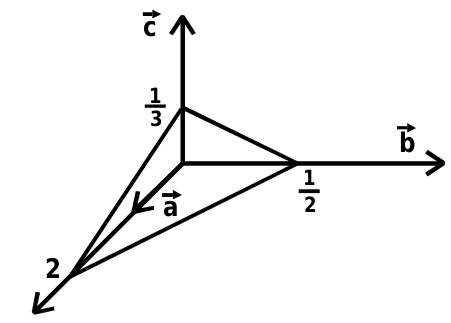
\includegraphics[width=0.3\textwidth]{../pics/miller.png}
	\caption{Bedeutung der Millerschen Indizes anhand eines Beispiels. Eingezeichnet sind eine Netzebene und der Koordinatenursprung mit seinen Achsen. \cite{Anleitung}}
	\label{pic:miller}
\end{figure}
In Abbildung \ref{pic:miller} schneidet eine Netzebene die Koordinatenachsen bei $2a$, $\nicefrac{1}{2}$ b und $\nicefrac{1}{3}$ c. Von diesen Zahlen nimmt man nun die Kehrwerte und multipliziert diese mit dem kleinsten gemeinsamen Vielfachen, damit man ganze Zahlen erhält. Die Millerschen Indizes wären in diesem Fall also $(hkl) = (146)$. Negative Zahlen werden mit einem Strich über der Zahl $-4 \rightarrow \bar{4}$ gekennzeichnet und wenn eine Achse gar nicht geschnitten wird (bzw. nur im Unendlichen), so ist der Indize $\nicefrac{1}{\infty}=0$.

Für orthogonale Kristallsysteme lässt sich der Netzebenabstand sehr einfach durch die Millerschen Indizes und der Gitterkonstanten a, b und c ausdrücken:
\begin{align}
	d &= \frac{1}{\sqrt{\frac{h^2}{a^2} + \frac{k^2}{b^2} + \frac{l^2}{c^2}}}
\end{align}
was sich für kubische Elementarzellen mit a = b = c weiter vereinfacht zu:\\
\begin{align}
	d &= \frac{a}{\sqrt{h^2 + k^2 + l^2}}
	\label{eq:gapMiller}
\end{align}

\subsection{Röntgenreflexion und Interferenz}
Wird ein Kristall Röntgenstrahlung ausgesetzt, so werden die Elektronenhüllen der Atome an den Gitterplätzen zu Schwingungen angeregt und emittieren ihrerseits die Strahlung wieder. Da die Gitterplätze räumlich streng periodisch angeordnet sind, kann dadurch Interferenz auftreten. In Abbildung \ref{eq:bragg} ist der geometrische Zusammenhang zum Gangunterschied $\Delta s$ dargestellt.
\begin{figure}[htbp]
	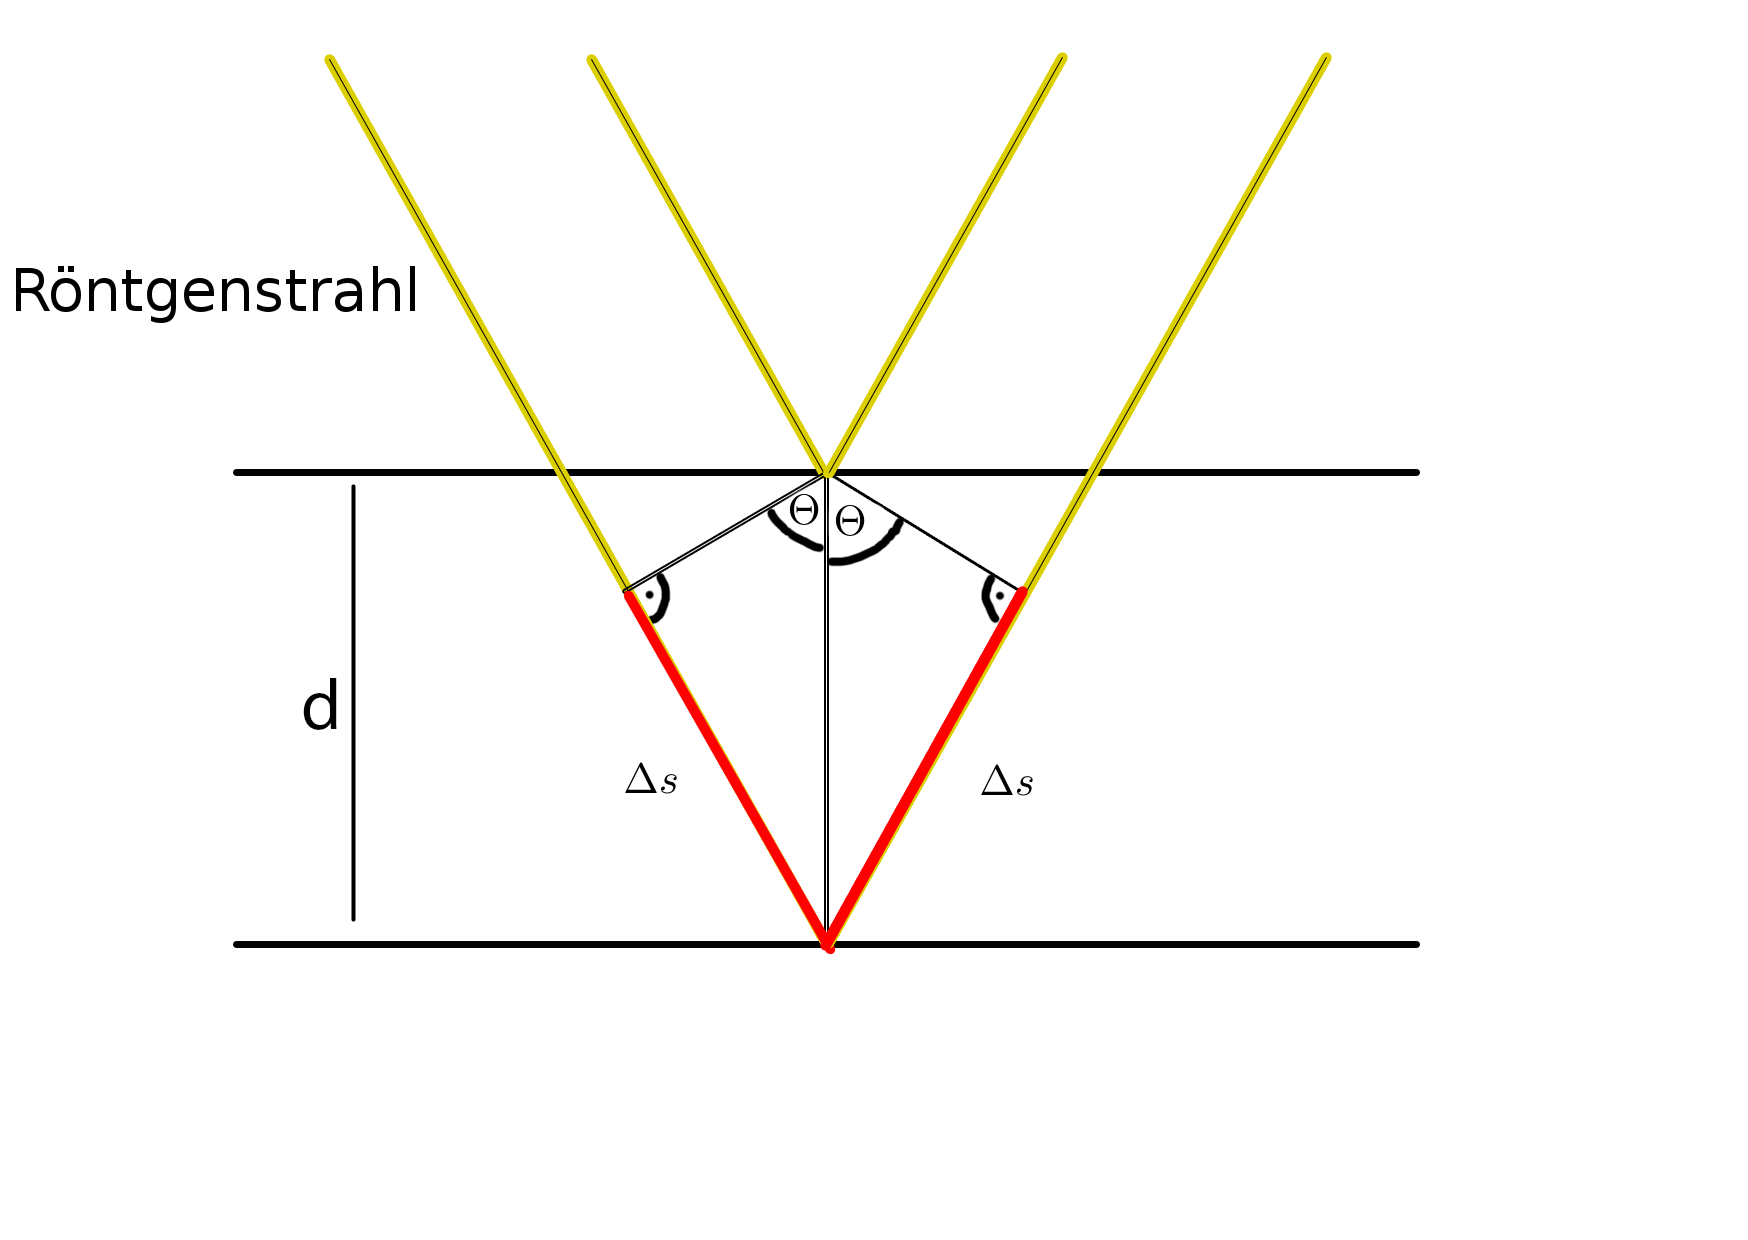
\includegraphics[width=0.6\textwidth]{../pics/bragg.png}
	\caption{Streuung der Röntgenstreuung an den Kristallebenen. Der Gangunterschied ist in rot dargestellt.\\
		Skizze: Jan Adam}
	\label{pic:bragg}
\end{figure}
Wenn dieser ein ganzzahliges Vielfaches der Wellenlänge $\lambda$ ist, so interferieren die Wellen konstruktiv und ein Röntgenreflex kann unter dem Winkel $\theta$ festgestellt werden. Zusammen mit dem Netzebenabstand $d$ lautet die Interferenzbedingung für konstruktive Interferenz an parallelen Netzebenen:
\begin{align}
 \lambda = 2 d \sin(\theta)
 \label{eq:bragg}
\end{align}
Dies ist die sog. Braggsche Bedingung. Es werden nun im Folgenden verschiedene Kristalle Röntgenstrahlung ausgesetzt um an Hand der Reflexionswinkel und mittels Gleichung \ref{eq:bragg} den Netzebenenabstand zu errechnen und dadurch Rückschlüsse auf das Probenmaterial zu ziehen. Beim hier verwendeten Debeye-Scherrer Verfahren wird anstelle eines einzelnen Einkristalls eine pulverisierte Probe verwendet. Durch die Zufällige Orientierung der Probenstückchen im Röntgenstrahl erfüllt stehts eine gewisse Anzahl der Kristallen die Bragg-Bedingung, so dass konstruktive Interferenz der Strahlung auftreten kann und sich der Filmstreifen an dieser Stelle schwarz färbt.

\section{Durchführung}
In diesem Versuch sollen die Elementarzellen eines Kristalls durch Röntgenreflexe untersucht werden.\\
Die Probe befindet sich dazu in einer komplett verdunkelten Filmdose, die nur zwei Öffnungen für den ein- und austretenden Röntgenstrahl hat. In der Mantelfläche ist ein Fotofilm angebracht, der sich durch die reflektierte Röntgenstrahlung schwarz färbt (siehe Abbildung \ref{pic:aufbau}). Mit diesem Filmstreifen können im Anschluss die Reflektionswinkel bestimmt werden. 
Die Proble wird präpariert, indem ein Kristall fein zerstäubt und auf ein Probenstäbchen aufgetragen wird.
\begin{figure}[htbp]
	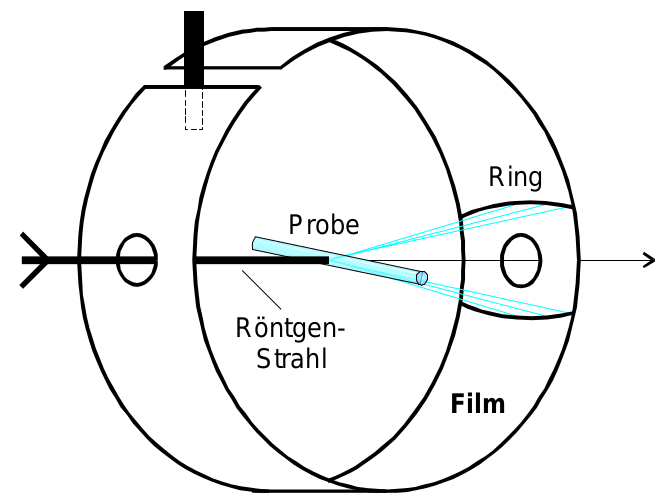
\includegraphics[width=0.6\textwidth]{../pics/aufbau.png}
	\caption{Im Versuch verwendeter Aufbau. Zusehen ist das zentrale Probenstäbchen, welches von den Röntgenstrahlen getroffen wird und Interferenzringe auf den Filmstreifen wirft.}
	\label{pic:aufbau}
\end{figure}
Die Probe wird deshalb zerstäubt, da konstruktive Interferenz nur auftritt, wenn die Röntgenstrahlung im Braggwinkel auf eine Netzebene trifft (also Gleichung \ref{eq:bragg} erfüllt ist). Ein Einkristall des Probenstoffs müsste daher während der Messung mehrmals gedreht werden, um alle Reflexe zu erhalten. Durch das Zerstäuben werden dagegen viele kleine Mikrokristalle erzeugt und zufällig ausgerichtet, so dass es zu jeder Netzebene immer einige Kristalle gibt, unter dem Braggwinkel getroffen werden. Daher werden alle möglichen Reflexe gleichzeitig erzeugt.\\
Um die Trefferquote weiter zu erhöhen, wird zudem das Probenstäbchen durch einen Motor langsam gedreht. 

Alle Mikrokristalle, die optimal getroffen werden und zur selben Netzebene gehören, erzeugen einen Kegel aus Röntgenstrahlen, der als Kreis auf dem Fotofilm sichtbar wird. Und aus dessen Öffnungswinkel der Netzebenenabstand bestimmt werden kann.

Die Messung wurde für zwei verschiedene Stoffe durchgeführt und anschließend wurden beide Filme in einer Dunkelkammer entwickelt. Im Folgenden werden die fertig entwickelten Streifen untersucht und die Öffnungswinkel der Röntgenreflexe abgelesen.  

\section{Auswertung}
\subsection{Bestimmung der Gitterkonstanten}
Mit einem Lineal werden entsprechend Abbildung \ref{pic:debyefilm} die Abstände $r_i$ der Beugungsringe zum Austrittsloch gemessen. Der 
Beugungswinkel kann nun mit $2\theta_i = r_i/R$ errechnet werden, wobei $R=57,4$ mm der Kammerradius ist. 
\begin{figure}[H]
 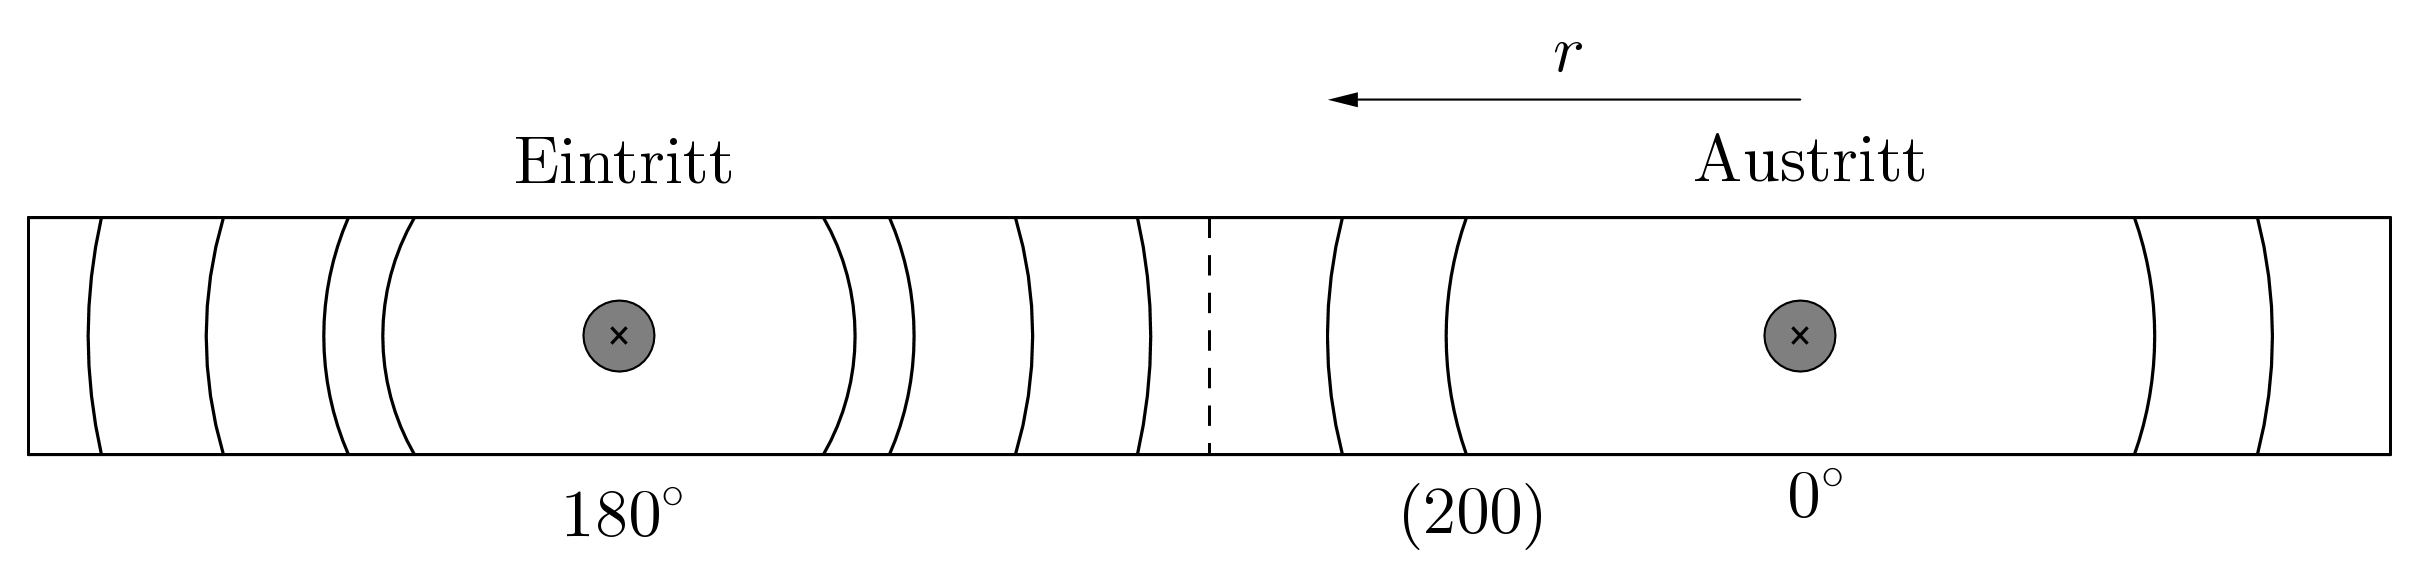
\includegraphics[width=\textwidth]{../pics/debyestreifen.jpg}
 \caption{Debye Filmaufnahme}
 \label{pic:debyefilm}
\end{figure}
\noindent Abhängig von der Gitterstruktur wie bcc ($h+k+l$ gerade), oder fcc ($hkl$, alle gerade oder ungerade),
wird der Reflex des niedrigsten Winkels $\theta_0$ an der ersten in Tabelle \ref{tab:hklstrukturen} aufgeführten Netzebene $(hkl)$
gestreut. 
Die experimentellen Strukturfaktoren $s^\text{exp}_i$ sind gegeben durch
\begin{align}
 s^\text{exp}_i = N^2_0 \frac{\sin^2(\theta_i)}{\sin^2(\theta_0)},
 \label{eq:structExp}
\end{align}
hervorgehend aus der Bragg-Gleichung \eqref{eq:bragg} und \eqref{eq:gapMiller}. Die Strukturen sc und CsCl haben für alle ebenen Reflexe, wobei CsCl
in bcc übergeht, wenn die Elemente in der CsCl-Struktur die gleichen Formfaktoren $f$ haben.
\begin{table}[t]
\begin{tabular}{cc|cccccc}
 $hkl$&$N^2$& sc &bcc & fcc & Di & CsCl &ZB./StS./Fl.\\
 \hline
 110&2&x&x&&&x&\\
 111&3&x&&x&x&x&x\\
 200&4&x&x&x&&x&x\\
 220&8&x&x&x&x&x&x\\
 310&10&x&x&&&x&\\
 311&11&x&&x&x&x&x\\
 222&12&x&x&x&&x&x\\
 400&16&x&x&x&x&x&x\\
 330&18&x&x&&&x&\\
 331&19&x&&x&x&x&x\\
 420&20&x&x&x&&x&x\\
 332&22&x&x&&&x&\\
 422&24&x&x&x&x&x&x\\
 510&26&x&x&&&x&\\
 511&27&x&&x&&x&x\\
 333&27&x&&x&x&x&x\\
 440&32&x&x&x&&x&x\\
 530&34&x&x&&&x&\\
 531&35&x&&x&&x&x\\
 442&36&x&x&x&x&x&x\\
\end{tabular}
\caption{Liste von Millerschen Indizes, die mindestens für eine Gitterstruktur einen Reflex (x) liefern. sc = simple cubic, bcc = body centered cubic, fcc =face centered cubic,
 Di = Diamant, CsCl = Cäsiumchlorid, ZB = Zinkblende, StS = Steinsalz, Fl = Flouritstruktur}
\label{tab:hklstrukturen}
\end{table}
\noindent  Nun werden die $(h_ik_il_i)$-Tripel
verrechnet zu
\begin{align}
 s^\text{theo}_i = h_i^2 + k_i^2 + l_i^2,
 \label{eq:structTheo}
\end{align}
mit den $s^\text{exp}$ verglichen und ihre akkumulierte Differenz $\Delta=\left(\frac{|s^\text{exp}-s^\text{theo}|}{N_\text{Ringe}}\right)$ möglichst gering gehalten unter Variation der Millerschen Indizes. Durch Ausschlussverfahren 
erschließt sich, um welche Gitterstruktur es sich handelt. Aus der Ähnlichkeit der Werte
aus Tabelle \ref{tab:messreihe1} für \textit{Metall 1} ist die bcc-Struktur zu bevorzugen. Für \textit{Salz 1} die StS-Struktur.
Damit kann man bereits den Gitterparameter $a$ berechnen als
\begin{align}
 a_i = \lambda\frac{\sqrt{s^\text{theo}_i}}{2\sin(\theta)}.
 \label{eq:gitterparameter}
\end{align}
mit $\lambda=0,154$ nm als Wellenlänge der Röntgenstrahlen. Die bisher angesprochenen Größen sind in den Tabellen 
\ref{tab:messreihe1} und \ref{tab:messreihe2} zu finden.

\begin{table}[H]
 \begin{tabular}{cccccc}
$r$ in mm&	$\theta$ in $\pi$& $s^\text{exp}$& $s^\text{theo}$ & MI &$a$ in $\mathring{A}$\\
\hline
45&	0.39&	2.0&	2&	110&	2.85 \\
65&	0.57&	3.9&	4&	200&	2.87\\
81&	0.71&	5.8&	6&	211&	2.91\\
97&	0.84&	7.7&	8&	220&	2.92\\
114&	0.99&	9.6&	10&	310&	2.91\\
135&	1.18&	11.7&	12&	222&	2.89\\
157&	1.37&	13.1&	14&	321&	2.94
 \end{tabular}
 \caption{Messwerte zur Metall 1. Für die bcc Struktur ist $\Delta=0.31$ und für fcc $\Delta=1.10$.}
 \label{tab:messreihe1}
\end{table}

\begin{table}[H]
 \begin{tabular}{cccccc}
$r$ in mm&	$\theta$ in $\pi$& $s^\text{exp}$& $s^\text{theo}$ & MI &$a$ in $\mathring{A}$\\
\hline
31&	0.27&	3.0&	3&	111&	5.00 \\
42&	0.37&	5.4&	4&	200&	4.31\\
51&	0.44&	7.8&	8&	220&	5.07\\
59&	0.51&	10.2&	11&	311&	5.20\\
66&	0.57&	12.5&	12&	222&	4.91\\
72&	0.63&	14.5&	16&	400&	5.25\\
86&	0.75&	19.6&	19&	331&	4.93\\
92&	0.80&	21.8&	20&	420&	4.80\\
98&	0.85&	23.9&	24&	422&	5.01\\
105&	0.91&	26.5&	27&	333&	5.06\\
117&	1.02&	30.6&	32&	440&	5.12\\
125&	1.09&	33.1&	35&	531&	5.15\\
151&	1.32&	39.5&	36&	600&	4.78\\
166&	1.45&	41.5&	40&	620&	4.91
 \end{tabular}
 \caption{Messwerte zur Salz 1. Für die bcc Struktur ist $\Delta=1.39$ und für fcc $\Delta=1.11$.}
 \label{tab:messreihe2}
\end{table}

\subsection{Korrektur zum Gitterparameter und Bestimmung der Proben}
Bei der Versuchsdurchführung treten zwei wesentliche, systematische Fehler auf. Zum einen ist eine Abhängigkeit des Gitterparameters vom Beugungswinkel
bemerkbar,
was im Wesentlichen der Absorbtion der Röntgenstrahlen geschuldet ist. Und zum anderen fallen Probenachse und Filmzylinderachse nicht perfekt zusammen.
Es zeigt sich, dass bei der Apparatur der Fehler $\Delta a$ näherungsweise von der Summe beider Fehler und linear von $\cos^2(\theta)$ abhängt. Mittels
linearer Regression durch \texttt{Python3} wird $a$ bei $\theta = 90^\circ$, also $\cos^2(\theta)=0$, als bester Wert angenommen (vgl. Abb. \ref{pic:fita1}, \ref{pic:fita2}). 


\begin{figure}[H]
	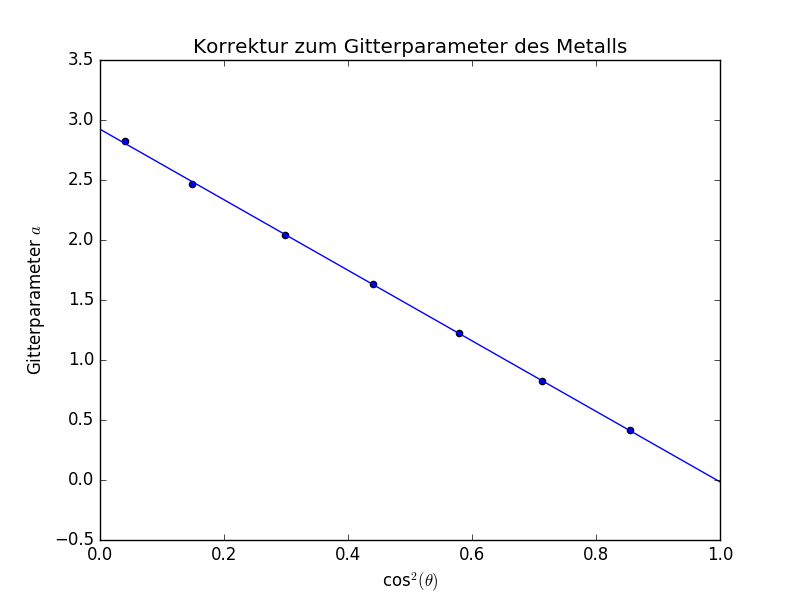
\includegraphics[width=0.7\textwidth]{../pics/a1.png}
	\caption{Korrigierter Wert für $a_\text{Metall}$ bei $\cos(\theta)=0$}
	\label{pic:fita1}
\end{figure}

\begin{figure}[H]
	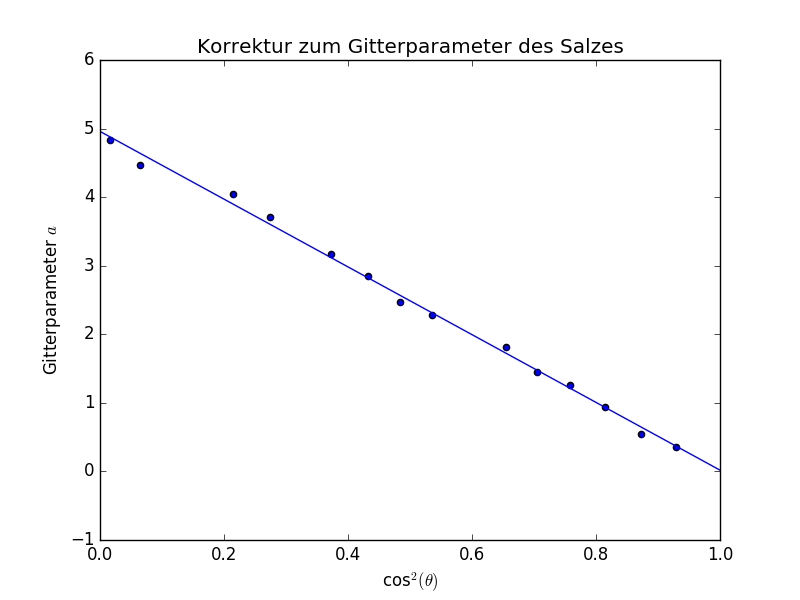
\includegraphics[width=0.7\textwidth]{../pics/a2.png}
	\caption{Korrigierter Wert für $a_\text{Salz}$ bei $\cos(\theta)=0$}
	\label{pic:fita2}
\end{figure}

\begin{align}
 a_\text{Metall} &= 2.93(10)\, \mathring{A} \\
 \nonumber
 a_\text{Salz} &= 5.00(23)\, \mathring{A} 
 \label{eq:latticeResults}
\end{align}

\noindent
\section{Diskussion}
Mit den ermittelten Werten für die Gitterkonstanten beider Proben, lassen sich nun jeweils Kandidaten finden, die infrage kommen.

\noindent Materialien mit einem Gitterparameter von $a_\text{Metall} = 2.93(10) \mathring{A}$ sind in Tabelle \ref{tab:matProb1} %4.64(163) früher
aufgeführt.

\begin{table}[H]
 \begin{tabular}{cc}
Material &$a$ in $\mathring{A}$\\
\hline
Fe&2.87\\ 
Cr& 2.88\\ 
V & 3.02\\  
 \end{tabular}
 \caption{Kandidaten für Metall 1 mit bcc-Struktur \cite{Gitterparameter}\cite{metall}}
 \label{tab:matProb1}
\end{table}
\noindent  Vanadium ist zwar im Fehlerbereich, ist aber schwer in Reinform zu bringen. Auch wenn es farblich zur Probe passen würde, schließen wir
es aus. Chrom und Eisen sind farblich ebenfalls passend. Chrom ist ähnlich wie, aber eher als Vanadium rein zu erhalten und Eisen ist recht einfach
zu erhalten. Mit Prüfung des Magnetismus der Probe könnte man feststellen, ob es sich bei der Experimentierprobe um Eisen oder Chrom handelt.

\noindent
Die NaCl-Struktur liefert Reflexe ähnlich der fcc-Struktur. Die Intesität variiert jedoch wenn die Miller-Indizes alle gerade
(die Formfaktoren der beiden Elemente $f_1$,$f_2$ werden in den Strukturfaktoren addiert) oder alle ungerade (sie werden subtrahiert) sind \cite{Azaroff}. Diese
Struktur wird von Salzen in Tabelle \ref{tab:matProb2} angenommen.
\begin{table}[H]
 \begin{tabular}{cc}
Material &$a$ in pm\\
\hline
AgF & 4.92\\ %gelb, ätzend, giftig
LiCl & 5.14\\ %weiß, 
SrO& 5.16\\ %weiß, ätzend
MgS & 5.20  %rötlich, ungefährlich
 \end{tabular}
 \caption{Kandidaten für die zweite Probe mit NaCl-Struktur \cite{Gitterparameter}\cite{Salz}}
 \label{tab:matProb2}

\end{table}
\noindent Silberflourid und Magnesiumsulfid passen beide farblich nicht zur weißen Probe. Weiterhin ist AgF ätzend und giftig. Strontiumoxid passt
zwar farblich ist jedoch ebenfalls ätzend, weshalb wir für die nicht weiter gesicherte Handhabe annehmen, dass sie nicht das Probenmaterial sind. 
Schließlich bleibt Lithiumchlorid als Kandidat im Bereich von $a_\text{Salz} = 5.00(23)\, \mathring{A} $, der farblich passt und keine weiteren Sicherheitsvorkehrungen erfordert, sofern er nicht als Lösung
vorliegt. 
\newpage
\begin{thebibliography}{xxx}
 \bibitem[1]{Anleitung}Versuchsanleitung: V41 Debye-Scherrer-Aufnahmen
 \bibitem[2]{Gitterparameter}Ashcroft N. and Mermin N.: \textit{Solid State Physics}, Harcourt, Inc. (1976) 
  \bibitem[3]{Azaroff}Azaroff,  L.V.  and  Buerger,  M.J.  \textit{The  Powder  Method  in  X-ray  Crystallography},  McGraw-Hill,  1958
  \bibitem[4]{Salz}West A.R. \textit{Basic Solid State Chemistry}  2nd edn. John Wiley \& Sons, Chichester, 1999
  \bibitem[5]{metall}Hermann K. \textit{Crystallography and Surface Structure: An Introduction for Surface Scientists and Nanoscientists}, WILEY-VCH Verlag GmbH \& Co. KGaA, 2011
\end{thebibliography}


% ========================================
%	Literaturverzeichnis
% ========================================

%\bibliographystyle{plainnat}			% Bibliographie-Style auswählen
%\bibliography{BIBDATEI}			% Literaturverzeichnis

%http://www.uni-mainz.de/FB/Physik/ATOS/Arbeiten/Schemies/Dissertation/node8.html (Zinkblende)
%http://www.tf.uni-kiel.de/matwis/amat/mw_for_et/kap_3/backbone/r3_2_2.html (Diamant)

% ========================================
%	Das Dokument endent
% ========================================

\end{document}
